% Chapter Template

\chapter{Software Requirement Specification} % Main chapter title

\label{Software Requirement Specification} % Change X to a consecutive number; for referencing this chapter elsewhere, use \ref{ChapterX}

\lhead{ \emph{Software Requirement Specification}} % Change X to a consecutive number; this is for the header on each page - perhaps a shortened title

%----------------------------------------------------------------------------------------
%	SECTION 1
%----------------------------------------------------------------------------------------

\section{Version}

\begin{tabular}{| p{1.5cm} | p{2cm} | p{9cm} | p{1.5cm} |}
	\hline
	Version & Date 		& Change & Author \\ \hline
	0.1 	& 20.09.2014 	& Setup document  										& JR \\ \hline
	0.2 	& 28.09.2014		& Add features										& JR \\ \hline
	0.3 	& 30.09.2014		& Change features, grammar, layout					& JR \\ \hline
	0.4 	& 02.10.2014		& Add overview of application/evaluation			& JR \\ \hline
	0.5 	& 04.10.2014		& Corrections evaluation 							& JR \\ \hline
	1.0 	& 05.10.2014		& Grammar, layout 									& JR \\ \hline
	1.1 	& 20.11.2014		& Fix FN definition									& JR \\ \hline

\end{tabular}

\section{Introduction}

\ref{Software Requirement Specification}


\subsection{Purpose}

The software requirement specification is providing all needed information to develop the context extraction framework and define all delivery objects. All interfaces to external components, input and output data, deployment considerations and quality attribute are well defined within this document.


\subsection{Scope}


The context extraction framework will perform automated text extraction on a set of HTML test data with two to three different text extraction algorithms. After measuring the performance of each algorithm, an output file with the measured results is generated.

%----------------------------------------------------------------------------------------
%	SECTION 2
%----------------------------------------------------------------------------------------

\section{General description}

\subsection{Operating Environment}

The operation environment for the text extraction framework is defined in this section.

\subsubsection{Local environment}

\begin{tabular}{| p{3cm} | p{3cm} |}
	\hline
	Ubuntu & 12.04 \\ \hline
	JDK & 1.7.X  \\ \hline
	Gradle & 1.11 \\ \hline
	Eclipse Keppler & 2.X \\ \hline
	git & 1.9.X \\ \hline
	python & 2.7.X \\ \hline

\end{tabular}


\subsubsection{Continuous Integration Environment}

\begin{tabular}{| p{3cm} | p{3cm} |}
	\hline
	Ubuntu & 12.04 \\ \hline
	Open JDK & 1.6.X  \\ \hline
	Open JDK & 1.7.X  \\ \hline
	Oracle JDK & 1.7.X \\ \hline
	Oracle JDK & 1.8.X  \\ \hline
	Gradle & 2.0 \\ \hline
	Travis CI &  \\ \hline
\end{tabular}



\subsection{Design and Implementation Constraints}

\subsubsection{User interface}
As parts of the text extraction framework may be implemented in a server environment at a later point in time and a user interface is not desired from the client, there will be no graphical user interface. The application is built, deployed and started by gradle. While the application is running, no interaction is needed. \cite{Reference1} \cite{CLEANEVAL:online}


\section{System Features}

This section specifies all system features. Each feature is specified more closely with multiple user stories. However, all the important information, such as external dependencies and output files, are defined in this chapter. The related user stories for each feature are located in the planning section.  



\begin{landscape}

\subsection{Basic functionality}
The following diagram and text describes the basic functionality of the application.

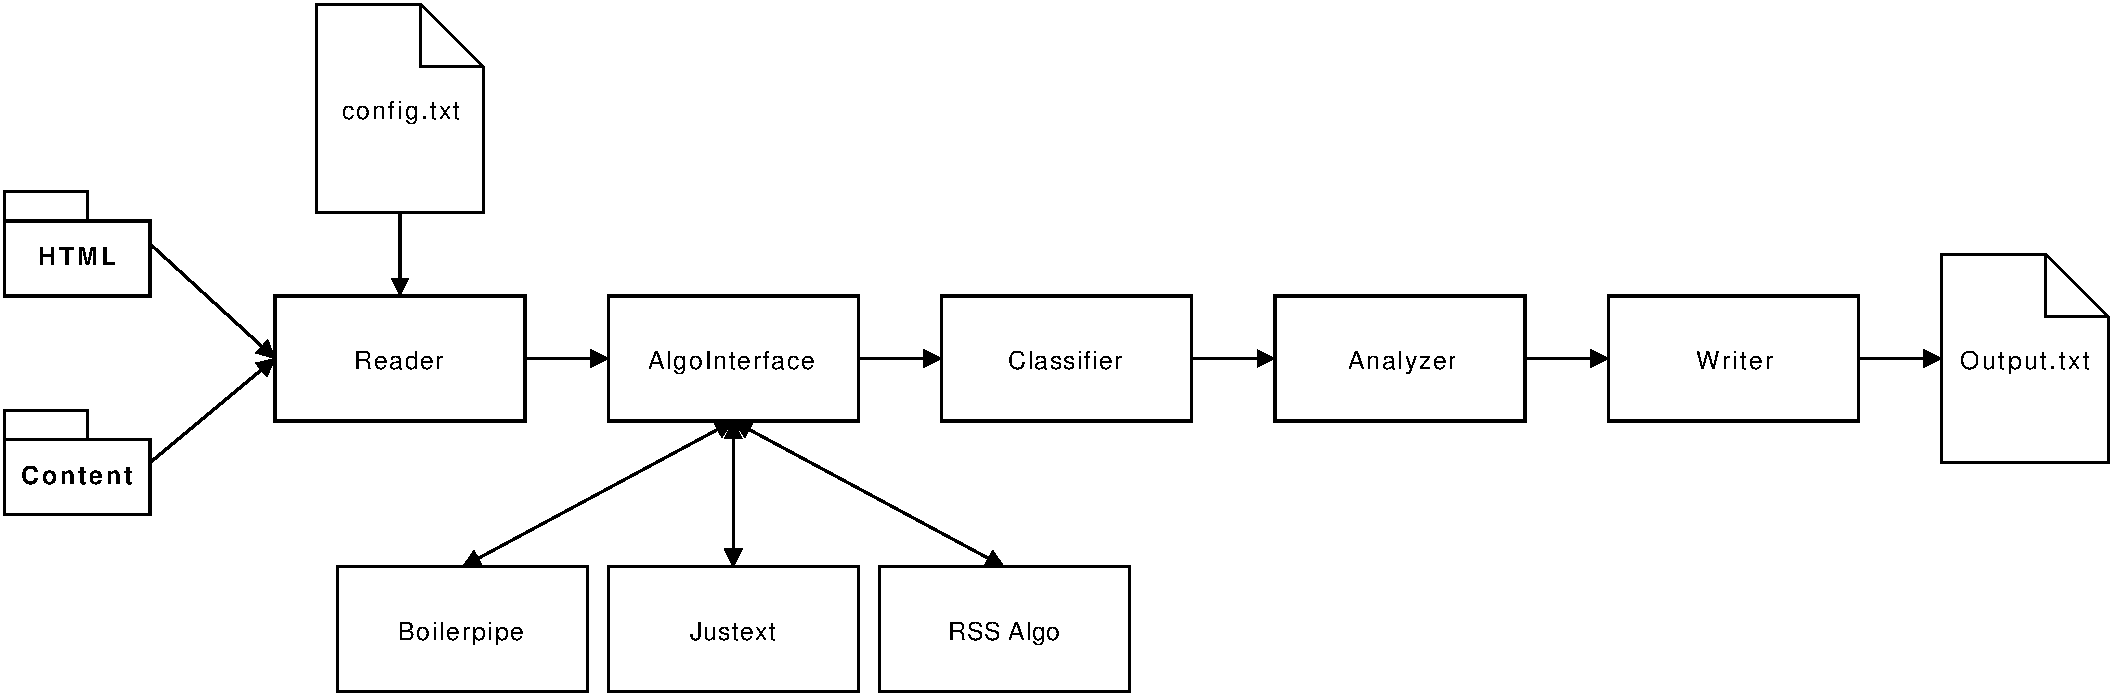
\includegraphics[width=24cm]{Figures/AppOverview.pdf}

There are two folders defined by the configuration file (config.txt). The HTML folder contains  HTML files of web pages. The content folder contains text files with the relevant content of the related HTML files. As soon as a test is started, the HTML file and the text file are read and the HTML file is extracted and classified with all the available algorithms. The result of the classification is then compared to the relevant content and performance data is generated. This performance data is then analyzed with statistical methods. 

\end{landscape}



\subsection{Overview}

	\begin{tabular}{ | p{0.5cm} | p{9cm} |p{2cm} |p{2.5cm} |}
	\hline
	\textbf{ID}	& \textbf{Name} 									& \textbf{Chapter}    											& \textbf{Relevance}	\\ \hline
	f1  		& Read configuration 								& \ref{subsec:Read configuration}  								& needed 				\\ \hline
	f2  		& Create test 										& \ref{subsec:Create test}										& needed 				\\ \hline
	f3  		& Integration Justext algorithm 					& \ref{subsec:Integration Justext algorithm} 					& needed 				\\ \hline
	f4  		& Integration Boilerpipe algorithm 					& \ref{subsec:Integration Boilerpipe algorithm}  				& needed 				\\ \hline
	f5  		& Evaluation and Implementation RSS feed algorithm 	& \ref{subsec:Evaluation and Implementation RSS feed algorithm} & nice to have			\\ \hline
	f6  		& Evaluation of classification text 				& \ref{subsec:Evaluation of classification text}				& needed 				\\ \hline
	f7  		& Evaluation of classification blocks 				& \ref{subsec:Evaluation of classification blocks}	  			& nice to have			\\ \hline
	f8  		& Analyze data 										& \ref{subsec:Analyze data}										& needed 				\\ \hline
	\end{tabular} \\



\subsubsection{Read configuration}
\label{subsec:Read configuration}

	\begin{tabular}{ | p{3cm} | p{12cm} |}
	\hline
	\textbf{Name} 				& Read configuration 				\\ \hline
	\textbf{Feature id} 		& f1 				\\ \hline
	\textbf{Description} 		& The text extraction framework is configurable with an external text file. The configuration file will contain following items:
							        \begin{itemize}
							        \item Path to folder with HTML files
							        \item Path to folder with text files
							        \item Path to folder with output files
							        \item Configuration for algorithms
							        \item etc.
						        \end{itemize} 
						        The configuration file location is defined as a relative path to the source directory and structured in a key value list: 

						        \lstinputlisting{Code/configTemplate.txt} \\ \hline
	\textbf{Relevance} 			& needed 			\\ \hline
	\textbf{Related stories} 	& tbd		\\ \hline
	\end{tabular} \\

\subsubsection{Create test}
\label{subsec:Create test}

	\begin{tabular}{ | p{3cm} | p{12cm} |}
	\hline
	\textbf{Name} 				& Create test \\ \hline
	\textbf{Feature id} 		& f2 \\ \hline
	\textbf{Description} 		& A test contains two input files which are an HTML file and a text file. They are located in the directories defined by the configuration. As soon as the test framework finds an HTML and a text file with the same name, the files are read and the test is started.\\ \hline
	\textbf{Relevance} 			& needed \\ \hline
	\textbf{Related stories} 	& tbd \\ \hline
	\end{tabular} \\

\subsubsection{Integration Justext algorithm}
\label{subsec:Integration Justext algorithm}

	\begin{tabular}{ | p{3cm} | p{12cm} |}
	\hline
	\textbf{Name} 				& Integration Justext algorithm \\ \hline
	\textbf{Feature id} 		& f3 \\ \hline
	\textbf{Description} 		& Justext is implemented in python. That is the reason why a service is needed to call the python script and get the extracted text or the extracted blocks.\\ \hline
	\textbf{Relevance} 			& needed \\ \hline
	\textbf{Related stories} 	& tbd \\ \hline
	\end{tabular} \\

\subsubsection{Integration Boilerpipe algorithm}
\label{subsec:Integration Boilerpipe algorithm}

	\begin{tabular}{ | p{3cm} | p{12cm} |}
	\hline
	\textbf{Name} 				& Integration Boilerpipe algorithm \\ \hline
	\textbf{Feature id} 		& f4 \\ \hline
	\textbf{Description} 		& Boilerplate is implemented in Java. An interfae is needed in order to call the Boilerplate component and get the extracted text or the extracted blocks.\\ \hline
	\textbf{Relevance} 			& needed \\ \hline
	\textbf{Related stories} 	& tbd \\ \hline
	\end{tabular} \\

\subsubsection{Evaluation and Implementation RSS feed algorithm}
\label{subsec:Evaluation and Implementation RSS feed algorithm}

\begin{tabular}{ | p{3cm} | p{12cm} |}
	\hline
	\textbf{Name} 				& Evaluation and implementation RSS feed algorithm \\ \hline
	\textbf{Feature id} 		& f5 \\ \hline
	\textbf{Description} 		& The basic idea of the RSS feed algorithm is to match the content of an HTML document with the related RSS feed and in doing so, define the relevant content. This needs to be evaluated, implemented and integrated into the text extraction framework.  \\ \hline
	\textbf{Relevance} 			& nice to have\\ \hline
	\textbf{Related stories} 	& tbd \\ \hline
	\end{tabular} \\

\subsubsection{Evaluation of classification text}
\label{subsec:Evaluation of classification text}

	\begin{tabular}{ | p{3cm} | p{12cm} |}
	\hline
	\textbf{Name} 				& Evaluation of classification \\ \hline
	\textbf{Feature id} 		& f6 \\ \hline
	\textbf{Description} 		& All the text extraction algorithms return an extracted document as text. This document needs to be checked for accuracy, which is achieved by comparing the result of the algorithms with the actual content. 
								\begin{itemize}
							        \item Check each classified block from the algorithms if its content can be found in the actual content
							        \item Categorize text as boilerplate or content
							        \item Insert results in an output text file
						        \end{itemize} 

						        Both the evaluation and classification are defined in more detail in section \ref{subsec:Evaluation of classification}.
						        \\ \hline

	\textbf{Relevance} 			& needed\\ \hline
	\textbf{Related stories} 	& tbd \\ \hline
	\end{tabular} \\


\subsubsection{Evaluation of classification blocks}
\label{subsec:Evaluation of classification blocks}

	\begin{tabular}{ | p{3cm} | p{12cm} |}
	\hline
	\textbf{Name} 				& Evaluation of classification blocks \\ \hline
	\textbf{Feature id} 		& f7 \\ \hline
	\textbf{Description} 		& A more detailed evaluation of the algorithms could be done if not only the text but also each block of an HTML file is classified. So as to achieve the more detailed evaluation, the implementation of Justext and Boilerpiple has to be adapted so that they return classified blocks instead of the extracted text. These blocks are afterwards compared with the actual content and classified. 
								\begin{itemize}
							        \item Check each classified block from the algorithms if its content can be found in the content file
							        \item Categorize all blocks as boilerplate or content
							        \item Insert the results in an output text file (structure output file: tbd)
						        \end{itemize} 
	Both the evaluation and classification are defined in more detail in section \ref{subsec:Evaluation of classification}.
	\\ \hline
	\textbf{Relevance} 			& nice to have\\ \hline
	\textbf{Related stories} 	& tbd \\ \hline
	\end{tabular} \\





\subsection{Analyze data}
\label{subsec:Analyze data}

	\begin{tabular}{ | p{3cm} | p{12cm} |}
	\hline
	\textbf{Name} 				& Analyze data \\ \hline
	\textbf{Feature id} 		& f8 \\ \hline
	\textbf{Description} 		&  From the results of the comparison further values can be evaluated for a better understanding of the results. These values are described in more detail in section \ref{subsec:Analytical values}.
								    \\ \hline
	\textbf{Relevance} 			& needed \\ \hline
	\textbf{Related stories} 	& tbd \\ \hline
	\end{tabular} \\

\subsection{Evaluation of classification}
\label{subsec:Evaluation of classification}


The general meaning of the expressions true positive, true negative, false positive and false negative related to the text extraction topic is shown in following table.

\begin{table}[h]
\begin{tabular}{|p{4cm} |p{5.5cm} |p{5.5cm} |}\hline
          								& \textbf{Classified as content} 	& \textbf{Classified as boilerplate} 	\\ \hline
\textbf{Actual content} 				& True positive (TP)				& False negative(FN)					\\ \hline
\textbf{Actual boilerplate} 			& False positive (FP)       		& True negative (TN)				 	\\ \hline
\end{tabular}
\end{table}

When the results are compared based on words, the expressions are interpreted as follows.

 \begin{table}[h]
\begin{tabular}{|p{4cm} |p{5.5cm} |p{5.5cm} |}
\hline         								& \textbf{Classified as content} 				& \textbf{Classified as boilerplate} 					\\ \hline
\textbf{Actual content} 				& Word classified as content by algorithm and is content		& Word classified as boilerplate by algorithm but is content		\\ \hline
\textbf{Actual boilerplate} 			& Word classified as content by algorithm but is boilerplate 	& Word classified as boilerplate by algorithm and is Boilerplate	\\ \hline
\end{tabular}
\end{table}

When the results are compared based on HTML blocks, the expressions are interpreted as follows.

 \begin{table}[h]
\begin{tabular}{|p{4cm} |p{5.5cm} |p{5.5cm} |}
\hline         							& \textbf{Classified as content} 								& \textbf{Classified as boilerplate} 								\\ \hline
\textbf{Actual content} 				& Block is classified as content by algorithm and is content		& Block is classified as boilerplate by algorithm but is content		\\ \hline
\textbf{Actual boilerplate} 			& Block is classified as content by algorithm but is boilerplate 	& Block is classified as boilerplate by algorithm and is boilerplate	\\ \hline
\end{tabular}
\end{table}

In conclusion, TP + FN is the correct outcome of the algorithm i.e. content classified as content and boilerplate as boilerplate. On the other hand, TN + FP is the wrong outcome of the algorithm i.e. content classified as boilerplate and boilerplate as content.



\subsection{Analytical values}
\label{subsec:Analytical values}

In this paragraph we use the notion of objects instead of word/block.
The results of the comparison deliver basic characteristics which can be used to calculate statistical values which help you analyze the test outcome.
										
\textbf{ Sensitivity / Recall /True positive rate / TPR / Hitrate }

Recall is the probability that a relevant document is retrieved in a search which in our case is

\begin{equation}
 Recall =\frac{TP}{TP + FN}
\end{equation}

correct classified content objects divided by the sum of all actual objects.

\textbf{Precision / True negative rate / TNR} 


Precision is the probability that a retrieved document is relevant which in our case is

\begin{equation}
 Presicion = \frac{TP}{TP + FP}
\end{equation}

correct classified content objects divided by the sum of all objects classified as content.

\textbf{F-measure / F1-score / F-score} 

F-measure is the harmonic mean of precision and recall which in our case is

\begin{equation}
Fmeasure =  2* \frac{presicion * recall}{presicion + recall}
\end{equation}

a measure of the test's accuracy.



\textbf{Fallout / False positive rate / FPR}

Fallout is the proportion of non-relevant objects that are retrieved out of all non-relevant objects available which in our case is

\begin{equation}
Fallout = \frac{FP}{FP + TN}
\end{equation}

%\textbf{Accuracy}

%\begin{equation}
%Accuracy =  \frac{TP+FN}{TP+TN+FP+FN}
%\end{equation}


\section{External Interface Requirements}

\subsection{Boilerpipe}

The boilerpipe algorithm is implemented in Java and the documentation is found under
\url{https://code.google.com/p/boilerpipe/}.

\subsection{justext}

The justext algorithem is implemented in python and the documentation is found under \url{https://code.google.com/p/justext/}. It is not yet defined how it will be integrated into the text extraction framework. See risk analysis for further information.


